% Options for packages loaded elsewhere
\PassOptionsToPackage{unicode}{hyperref}
\PassOptionsToPackage{hyphens}{url}
\PassOptionsToPackage{dvipsnames,svgnames,x11names}{xcolor}
%
\documentclass[
  10pt,
  letterpaper,
  DIV=11,
  numbers=noendperiod]{scrartcl}

\usepackage{amsmath,amssymb}
\usepackage{iftex}
\ifPDFTeX
  \usepackage[T1]{fontenc}
  \usepackage[utf8]{inputenc}
  \usepackage{textcomp} % provide euro and other symbols
\else % if luatex or xetex
  \usepackage{unicode-math}
  \defaultfontfeatures{Scale=MatchLowercase}
  \defaultfontfeatures[\rmfamily]{Ligatures=TeX,Scale=1}
\fi
\usepackage{lmodern}
\ifPDFTeX\else  
    % xetex/luatex font selection
\fi
% Use upquote if available, for straight quotes in verbatim environments
\IfFileExists{upquote.sty}{\usepackage{upquote}}{}
\IfFileExists{microtype.sty}{% use microtype if available
  \usepackage[]{microtype}
  \UseMicrotypeSet[protrusion]{basicmath} % disable protrusion for tt fonts
}{}
\makeatletter
\@ifundefined{KOMAClassName}{% if non-KOMA class
  \IfFileExists{parskip.sty}{%
    \usepackage{parskip}
  }{% else
    \setlength{\parindent}{0pt}
    \setlength{\parskip}{6pt plus 2pt minus 1pt}}
}{% if KOMA class
  \KOMAoptions{parskip=half}}
\makeatother
\usepackage{xcolor}
\setlength{\emergencystretch}{3em} % prevent overfull lines
\setcounter{secnumdepth}{5}
% Make \paragraph and \subparagraph free-standing
\makeatletter
\ifx\paragraph\undefined\else
  \let\oldparagraph\paragraph
  \renewcommand{\paragraph}{
    \@ifstar
      \xxxParagraphStar
      \xxxParagraphNoStar
  }
  \newcommand{\xxxParagraphStar}[1]{\oldparagraph*{#1}\mbox{}}
  \newcommand{\xxxParagraphNoStar}[1]{\oldparagraph{#1}\mbox{}}
\fi
\ifx\subparagraph\undefined\else
  \let\oldsubparagraph\subparagraph
  \renewcommand{\subparagraph}{
    \@ifstar
      \xxxSubParagraphStar
      \xxxSubParagraphNoStar
  }
  \newcommand{\xxxSubParagraphStar}[1]{\oldsubparagraph*{#1}\mbox{}}
  \newcommand{\xxxSubParagraphNoStar}[1]{\oldsubparagraph{#1}\mbox{}}
\fi
\makeatother


\providecommand{\tightlist}{%
  \setlength{\itemsep}{0pt}\setlength{\parskip}{0pt}}\usepackage{longtable,booktabs,array}
\usepackage{calc} % for calculating minipage widths
% Correct order of tables after \paragraph or \subparagraph
\usepackage{etoolbox}
\makeatletter
\patchcmd\longtable{\par}{\if@noskipsec\mbox{}\fi\par}{}{}
\makeatother
% Allow footnotes in longtable head/foot
\IfFileExists{footnotehyper.sty}{\usepackage{footnotehyper}}{\usepackage{footnote}}
\makesavenoteenv{longtable}
\usepackage{graphicx}
\makeatletter
\def\maxwidth{\ifdim\Gin@nat@width>\linewidth\linewidth\else\Gin@nat@width\fi}
\def\maxheight{\ifdim\Gin@nat@height>\textheight\textheight\else\Gin@nat@height\fi}
\makeatother
% Scale images if necessary, so that they will not overflow the page
% margins by default, and it is still possible to overwrite the defaults
% using explicit options in \includegraphics[width, height, ...]{}
\setkeys{Gin}{width=\maxwidth,height=\maxheight,keepaspectratio}
% Set default figure placement to htbp
\makeatletter
\def\fps@figure{htbp}
\makeatother
% definitions for citeproc citations
\NewDocumentCommand\citeproctext{}{}
\NewDocumentCommand\citeproc{mm}{%
  \begingroup\def\citeproctext{#2}\cite{#1}\endgroup}
\makeatletter
 % allow citations to break across lines
 \let\@cite@ofmt\@firstofone
 % avoid brackets around text for \cite:
 \def\@biblabel#1{}
 \def\@cite#1#2{{#1\if@tempswa , #2\fi}}
\makeatother
\newlength{\cslhangindent}
\setlength{\cslhangindent}{1.5em}
\newlength{\csllabelwidth}
\setlength{\csllabelwidth}{3em}
\newenvironment{CSLReferences}[2] % #1 hanging-indent, #2 entry-spacing
 {\begin{list}{}{%
  \setlength{\itemindent}{0pt}
  \setlength{\leftmargin}{0pt}
  \setlength{\parsep}{0pt}
  % turn on hanging indent if param 1 is 1
  \ifodd #1
   \setlength{\leftmargin}{\cslhangindent}
   \setlength{\itemindent}{-1\cslhangindent}
  \fi
  % set entry spacing
  \setlength{\itemsep}{#2\baselineskip}}}
 {\end{list}}
\usepackage{calc}
\newcommand{\CSLBlock}[1]{\hfill\break\parbox[t]{\linewidth}{\strut\ignorespaces#1\strut}}
\newcommand{\CSLLeftMargin}[1]{\parbox[t]{\csllabelwidth}{\strut#1\strut}}
\newcommand{\CSLRightInline}[1]{\parbox[t]{\linewidth - \csllabelwidth}{\strut#1\strut}}
\newcommand{\CSLIndent}[1]{\hspace{\cslhangindent}#1}

\usepackage{braket}
\usepackage{amsmath}
\DeclareMathOperator{\tr}{tr}
\DeclareMathOperator{\diag}{diag}
\newcommand{\RWA}{\textrm{RWA}}
\newcommand{\lab}{\textrm{lab}}
\newcommand{\Hilbert}{\mathcal{H}}
\newcommand{\HilbertS}{\mathcal{H}_{\!S}}
\newcommand{\HilbertI}{\mathcal{H}_{\!I}}
\newcommand{\HilbertGE}{\mathcal{H}_{\!GE}}
\newcommand{\HilbertO}{\mathcal{H}_{\!O}}
\newcommand{\HilbertOS}{\mathcal{H}_{\!OS}}
\newcommand{\HilbertM}{\mathcal{I}_{\!M}}
\newcommand{\HilbertG}{\mathcal{I}_{\!G}}
\newcommand{\HilbertE}{\mathcal{I}_{\!E}}
\newcommand{\ketbra}[2]{\ket{#1}\!\bra{#2}}
\KOMAoption{captions}{tableheading}
\makeatletter
\@ifpackageloaded{caption}{}{\usepackage{caption}}
\AtBeginDocument{%
\ifdefined\contentsname
  \renewcommand*\contentsname{Table of contents}
\else
  \newcommand\contentsname{Table of contents}
\fi
\ifdefined\listfigurename
  \renewcommand*\listfigurename{List of Figures}
\else
  \newcommand\listfigurename{List of Figures}
\fi
\ifdefined\listtablename
  \renewcommand*\listtablename{List of Tables}
\else
  \newcommand\listtablename{List of Tables}
\fi
\ifdefined\figurename
  \renewcommand*\figurename{Figure}
\else
  \newcommand\figurename{Figure}
\fi
\ifdefined\tablename
  \renewcommand*\tablename{Table}
\else
  \newcommand\tablename{Table}
\fi
}
\@ifpackageloaded{float}{}{\usepackage{float}}
\floatstyle{ruled}
\@ifundefined{c@chapter}{\newfloat{codelisting}{h}{lop}}{\newfloat{codelisting}{h}{lop}[chapter]}
\floatname{codelisting}{Listing}
\newcommand*\listoflistings{\listof{codelisting}{List of Listings}}
\makeatother
\makeatletter
\makeatother
\makeatletter
\@ifpackageloaded{caption}{}{\usepackage{caption}}
\@ifpackageloaded{subcaption}{}{\usepackage{subcaption}}
\makeatother
\ifLuaTeX
  \usepackage{selnolig}  % disable illegal ligatures
\fi
\usepackage{bookmark}

\IfFileExists{xurl.sty}{\usepackage{xurl}}{} % add URL line breaks if available
\urlstyle{same} % disable monospaced font for URLs
\hypersetup{
  pdftitle={Generalized Hamiltonian for multiple ¹³C atoms around an NV center},
  pdfauthor={Michael Goerz},
  colorlinks=true,
  linkcolor={blue},
  filecolor={Maroon},
  citecolor={Blue},
  urlcolor={Blue},
  pdfcreator={LaTeX via pandoc}}

\title{Generalized Hamiltonian for multiple ¹³C atoms around an NV
center}
\author{Michael Goerz}
\date{January 28, 2026}

\begin{document}
\maketitle

For the purpose of implementing a very general numerical model of the
interaction of the nuclear spin of one or more ¹³C atoms with the
electronic spin of a single NV center in diamond in a private
\texttt{C13NV} Julia package, we extensively discuss the Hamiltonian and
Liouvillian for the system in full generality. Within \texttt{C13NV},
the construction is encapsulated in a \texttt{make\_nv\_system}
function, that receives various system parameters and returns a
Hamiltonian or Liouvillian (a
\texttt{QuantumPropagators.Generators.Generator} instance) along with a
list of labels (each label a tuple of strings).

We discuss first the high-level structure of the Hilbert space
(Section~\ref{sec-hilbert-structure}) and the Hamiltonian/Liouvillian
(Section~\ref{sec-hamiltonian-structure}) before deriving the operators
in detail. Section~\ref{sec-lab} lists the lab frame Hamiltonian and
defines the spin operators for the electronic and nuclear spins.
Section~\ref{sec-rwa} transforms the lab frame Hamiltonian into the
rotating frame. This yields one possible Hamiltonian to use numerically
(\texttt{frame\ =\ :rwa}). Section~\ref{sec-diag} goes further by
analytically diagonalizing the hyperfine interaction between the nuclear
spin and the electronic spin of the NV center. This yields an
alternative form the Hamiltonian (\texttt{frame\ =\ :diag}), which
allows for a better understanding of avoided Landau-Zener crossings,
discussed in Section~\ref{sec-lz}. Lastly, Section~\ref{sec-dissipation}
describes the Lindblad operators for the full dissipative model.

\section{Structure of the Hilbert space}\label{sec-hilbert-structure}

\begin{itemize}
\tightlist
\item
  The optical Hilbert space is \(\HilbertO\) with levels \(\ket{G}\),
  \(\ket{E}\), \(\ket{M}\). The Hilbert space may be truncated to
  \(\ket{G}\) is the parameter \texttt{Λ} representing \(\Lambda(t)\) is
  passed as \texttt{nothing}. Note that \texttt{Λ\ =\ 0.0} is possible
  to force inclusion of all optical levels.
\item
  The Hilbert space of the NV center electronic spin is \(\HilbertS\)
  with levels \(\ket{+1}\), \(\ket{0}\), \(\ket{-1}\). The \(\ket{-1}\)
  level is truncated if the \texttt{Ω}\(_{-}\) parameter representing
  \(\Omega_{-}(t)\) is given as \texttt{nothing}, and likewise for
  \(\ket{+1}\) and \texttt{Ω}\(_{+}\). Either \texttt{Ω}\(_{+}\) or
  \texttt{Ω}\(_{-}\) can be passed as \texttt{0.0} to force inclusion of
  the level.
\item
  The nuclear spin of each surrounding C13 is a TLS with Hilbert space
  \(\HilbertI^{(n)}\) spanned by the states \(\ket{\uparrow}\),
  \(\ket{\downarrow}\). These get tensored into a \(2^N\)-dimensional
  spin space
  \(\HilbertI = \HilbertI^{(1)} \otimes \dots \otimes \HilbertI^{(N)}\);
  for \(N=2\): \(\ket{\uparrow\uparrow}\), \(\ket{\uparrow\downarrow}\),
  \(\ket{\downarrow\uparrow}\), \(\ket{\downarrow\downarrow}\) etc. for
  larger \(N\).
\end{itemize}

The structure of the full Hilbert space is a little bit tricky, since
the meta-stable state \(\ket{M}\) does not distinguish between different
electronic-spin degrees of freedom, and thus the three Hilbert spaces
are not simply tensored. Instead,

\begin{equation}\phantomsection\label{eq-Hilbert-space-structure}{
\begin{split}
\Hilbert
&= \HilbertG \otimes \HilbertS \otimes \HilbertI \; \oplus \; \HilbertE \otimes \HilbertS \otimes \HilbertI  \; \oplus \; \HilbertM \otimes \HilbertI \\
&= (\HilbertG \oplus \HilbertE) \otimes \, \HilbertS \, \otimes \, \HilbertI \; \oplus \; \HilbertM \, \otimes \, \HilbertI \\
&= \underbrace{((\HilbertG \oplus \HilbertE) \otimes \, \HilbertS \, \oplus \, \HilbertM)}_{\equiv \HilbertOS} \, \otimes \, \HilbertI\,,
\end{split}
}\end{equation}

where \(\HilbertG\), \(\HilbertE\), and \(\HilbertM\) are the (trivial)
one-dimensional Hilbert spaces consisting only of the optical levels
\(\ket{G}\), \(\ket{E}\), and \(\ket{M}\), respectively. \(\HilbertS\)
is the Hilbert space of the electronic spin, spanned by the three levels
\(\ket{+1}\), \(\ket{0}\), \(\ket{-1}\) (or a truncation thereof). We
may define
\(\HilbertOS = ((\HilbertG \oplus \HilbertE) \otimes \, \HilbertS \, \oplus \, \HilbertM)\)
in the third line of Equation~\ref{eq-Hilbert-space-structure} as the
combined Hilbert space for the optical and electronic-spin degree of
freedom, with the basis \(\ket{G,+1}\), \(\ket{G,0}\), \(\ket{G,-1}\),
\(\ket{E,+1}\), \(\ket{E,0}\), \(\ket{E,-1}\), \(\ket{M}\). The
structure in lines 2 and 3 of Equation~\ref{eq-Hilbert-space-structure}
is particularly helpful for constructing the relevant Lindblad operators
in the full (optical) system.

\section{Structure of the Hamiltonian and
Liouvillian}\label{sec-hamiltonian-structure}

The transitions in the electronic spin states of the NV center
\(\ket{+1}\), \(\ket{0}\), \(\ket{-1} \in \HilbertS\) are driven by a
microwave (MW) field

\begin{equation}\phantomsection\label{eq-combined-mw-field}{
\frac{1}{\sqrt{2}} \Omega(t) =
    \Omega_{-}(t) \cos(\omega_{-} t + \phi_{-}(t))
    + \Omega_{+}(t) \cos(\omega_{+} t + \phi_{+}(t))\,,
}\end{equation}

where the factor \(\frac{1}{\sqrt{2}}\) is to compensate the
normalization factor in the \(\hat{S}_x\) operator, see below in
Section~\ref{sec-lab}. In a two-color rotating frame for the central
frequencies \(\omega_{\pm}\), this results in four independent control
fields:

\begin{enumerate}
\def\labelenumi{\arabic{enumi}.}
\tightlist
\item
  \(\omega_{-}(t) \equiv \frac{d\phi_{-}(t)}{dt}\), the deviation
  (dynamic shift) from the central frequency \(\omega_{-}\). Note that
  we use both the time-dependent \(\omega_{-}(t)\) and the
  time-independent \(\omega_{-}\) with different meanings.
\item
  \(\omega_{+}(t) \equiv \frac{d\phi_{+}(t)}{dt}\), the deviation
  (dynamic shift) from the central frequency \(\omega_{+}\)
\item
  \(\Omega_{-}(t)\), the envelope for the amplitude driving the
  \(\ket{-1} \leftrightarrow \ket{0}\) transition
\item
  \(\Omega_{+}(t)\), the envelope for the amplitude driving the
  \(\ket{0} \leftrightarrow \ket{+1}\) transition
\end{enumerate}

Within the \texttt{QuantumControl.jl} framework, the system Hamiltonian
is expressed in the nested-list format

\begin{equation}\phantomsection\label{eq-nested-list}{
\hat{H} = [\hat{H_0}, [\hat{H}_{\omega_{-}}, \omega_{-}(t)], [\hat{H}_{\omega_{+}}, \omega_{+}(t)], [\hat{H}_{\Omega_{-}}, \Omega_{-}(t)], [\hat{H}_{\Omega_{+}}, \Omega_{+}(t)]]
}\end{equation}

with the drift Hamiltonian \(\hat{H_0}\), the control Hamiltonians
\(\hat{H}_{\omega_{-}}\), \(\hat{H}_{\omega_{+}}\),
\(\hat{H}_{\Omega_{-}}\), and \(\hat{H}_{\Omega_{+}}\), and the controls
listed above.

Construction of the Hamiltonian proceeds as follows:

\begin{enumerate}
\def\labelenumi{\arabic{enumi}.}
\item
  Construct spin operators for the appropriately truncated Hilbert space
  \(\HilbertS\), as well as \(\HilbertI^{(n)}\)
\item
  Construct the parts of Equation~\ref{eq-combined-mw-field}
  \(\in \HilbertS \otimes \HilbertI\) according to
  Equation~\ref{eq-rwa-hamiltonian-nested-list} if
  \texttt{frame\ =\ :rwa}, see Section~\ref{sec-rwa}, or
  Equation~\ref{eq-hamiltonian-diagonal-nested-list} if
  \texttt{frame\ =\ :diag}, see Section~\ref{sec-diag}
\item
  If the full optical Hilbert space \(\HilbertO\) is required
  (\texttt{Λ} is given), extend each operator into the full \(\Hilbert\)
  according to

  \begin{equation}\phantomsection\label{eq-hamiltonian-extension}{
  \hat{H}_{n} \rightarrow (𝟙_G \otimes \hat{H}_n) \,\oplus\, \underbrace{(𝟙_E \otimes 𝟘_S \otimes 𝟘_I) \,\oplus\, (𝟙_M \otimes 𝟘_I)}_{\text{padding}}
  }\end{equation}

  cf.~the first line of Equation~\ref{eq-Hilbert-space-structure}, with
  the trivial \(𝟙_G =  𝟙_E  = 𝟙_M = 1\). That is, we are simply padding
  the Hamiltonian with zeros to reach the size of the full Hilbert
  space. The choice of \(𝟘_S\) and \(𝟘_I\) reflects the fact that there
  are no coherent dynamics in the \(\ket{E}\) and \(\ket{M}\) manifolds.
\end{enumerate}

The \texttt{make\_nv\_system} function returns a Liouvillian if
\texttt{Λ} is given, or if decay rates \(\gamma_{\pm 1}\) for the
spontaneous decay in the electronic spin levels is given with a decay
rate \(> 0\). The incoherent drive with \texttt{Λ} is time-dependent,
and must be set up specially, see Section~\ref{sec-dissipation} for
details.

\section{Lab Frame Hamiltonian for the Ground State
Manifold}\label{sec-lab}

We are considering here the Hamiltonian of a single electronic spin
described in the ground-state manifold \(\ket{G}\) by the spin operators
\(\hat{\mathbf{S}} = (\hat{S}_x, \hat{S}_y, \hat{S}_z)\) and \(N\)
nuclear spins described by
\(\hat{\mathbf{I}}^{(n)} = (\hat{I}^{(n)}_x, \hat{I}^{(n)}_y, \hat{I}^{(n)}_z)\),
with the element \(A_{i,j}^{(n)}\) of the hyperfine tensor giving the
strength of the interaction between the \(j = x,y,z\) components of the
\(n\)'th nuclear spin and the \(i = x,y,z\) component of the electronic
spin. The full Hamiltonian has the form
~{[}\citeproc{ref-AjoySA2018}{1},\citeproc{ref-MultiCarbon.jl}{2}{]},

\begin{equation}\phantomsection\label{eq-lab-hamiltonian}{
\hat{H}_{\lab} = D \hat{S}_z^2 - \gamma_e \mathbf{B} \cdot \hat{\mathbf{S}} + \sum_{n=1}^{N} \left( \sum_{\substack{i,j\\=x, y, z}} A^{(n)}_{i,j} (\hat{S}_i \otimes \hat{I}^{(n)}_j) - \gamma_c \mathbf{B} \cdot \hat{\mathbf{I}}^{(n)}
\right) + \Omega(t) \hat{S}_x\,,
}\end{equation}

with \(\Omega(t)\) given by Equation~\ref{eq-combined-mw-field}, the
electronic spin energy \(D \approx\) 3 GHz, the electron gyromagnetic
ratio \(\gamma_e =\) 2.8 MHz/G, the nuclear gyromagnetic ratio
\(\gamma_c =\) 1.07 kHz/G, and the hyperfine tensor \(A^{(n)}\)
mediating the interaction between the n-th carbon nuclear spin and the
electronic spin of the NV center. The spin operators for the electronic
spin are those for a spin-1 particle, with quantum numbers
\((+1, 0, -1)\), cf.~the \(\hat{S}_z\) operator:

\[
\hat{S}_x = \frac{1}{\sqrt{2}}\begin{pmatrix}
    0 & 1 & 0 \\
    1 & 0 & 1 \\
    0 & 1 & 0
\end{pmatrix}\,,\quad
\hat{S}_y = \frac{1}{\sqrt{2}}\begin{pmatrix}
    0 & -i &  0 \\
    i &  0 & -i \\
    0 &  i &  0
\end{pmatrix}\,,\quad
\hat{S}_z = \begin{pmatrix}
    1 & 0 &   0 \\
    0 & 0 &   0 \\
    0 & 0 &  -1
\end{pmatrix}\,,\quad
𝟙_S = \begin{pmatrix}
    1 & 0 &  0 \\
    0 & 1 &  0 \\
    0 & 0 &  1
\end{pmatrix}\,.
\]

If were are only going to drive one of the \(-1 \leftrightarrow 0\) or
\(0 \leftrightarrow +1\) transitions, we can simply truncate the Hilbert
space by cutting the above matrices to from \(3 \times 3\) to
\(2 \times 2\).

The nuclear spin is spin-\(\frac{1}{2}\), and thus, \[
\hat{I}_x^{(n)} = \frac{1}{2}\begin{pmatrix}
    0 & 1 \\
    1 & 0
\end{pmatrix}\,,\qquad
\hat{I}_y^{(n)} = \frac{1}{2}\begin{pmatrix}
    0 & -i \\
    i &  0
\end{pmatrix}\,,\qquad
\hat{I}_z^{(n)} = \frac{1}{2}\begin{pmatrix}
    1 &   0 \\
    0 &  -1
\end{pmatrix}\,,\qquad
𝟙_I^{(n)} = \begin{pmatrix}
    1 & 0 \\
    0 & 1
\end{pmatrix}\,,
\] with eigenstates labeled \(\ket{\uparrow}\) and \(\ket{\downarrow}\).

The magnetic field vector is

\begin{equation}\phantomsection\label{eq-magnetic-field-vector}{
\mathbf{B} = B \begin{pmatrix}
    \sin(\theta) \cos(\phi)\\
    \sin(\theta) \sin(\phi)\\
    \cos(\theta)
    \end{pmatrix}
}\end{equation}

with the azimuthal angle \(\theta\), the polar angle \(\phi\), and the
field-strength \(B\). We will assume \(\theta = 0\), but there is no
need to restrict a numerical model to a magnetic field not aligned with
the \(z\)-axis defined by the NV center. In
Equation~\ref{eq-lab-hamiltonian}, operators are implicitly tensored
with the identity operator of all other subspaces.

\section{Microwave Field Rotating Wave Approximation}\label{sec-rwa}

To simplify the numerical model, and to remove the fast oscillations
\(\omega_{+}\) and \(\omega_{-}\), we transform the Hamiltonian to a
rotating frame and apply the rotating wave approximation (RWA). The main
result of this section is Equation~\ref{eq-rwa-hamiltonian}.

The rotating frame is defined by the operator

\begin{equation}\phantomsection\label{eq-U-RWA}{
\hat{U}_{\RWA}(t)
= \diag\left[\;
\exp[i \omega_{+} t + \phi_{+}(t)], \quad
1, \quad
\exp[i \omega_{-} t + \phi_{-}(t)]
\;\right]
}\end{equation}

in the electronic spin subspace. The wave function in the rotating frame
is defined as
\(\ket{\tilde{\Psi}(t)} = \hat{U}_{\RWA}(t) \ket{\Psi(t)}\). The
Hamiltonian in the rotating frame is

\begin{equation}\phantomsection\label{eq-H-RWA-general}{
\hat{H}_{\RWA} = i \hbar \dot{U}_{\RWA} \hat{U}_{\RWA}^\dagger + \hat{U}_{\RWA} \hat{H}_{\lab} \hat{U}_{\RWA}^\dagger
}\end{equation}

We again have the implicit tensor product, i.e.~in the full Hilbert
space, Equation~\ref{eq-H-RWA-general} is more properly written with
\(\hat{U}_{\RWA} \rightarrow \hat{U}_{\RWA} \otimes 𝟙_I\). It is helpful
to explicitly consider the transformation in the
electronic-spin-subspace within this tensor structure. For the first
term in Equation~\ref{eq-H-RWA-general},

\begin{equation}\phantomsection\label{eq-RWA-term1}{
i \hbar \left(\frac{\partial}{\partial t}(\hat{U}_{\RWA} \otimes 𝟙_I)\right)\left(\hat{U}_{\RWA} \otimes 𝟙_I \right)^\dagger
= (i \hbar \dot{U}_{\RWA} \hat{U}_{\RWA}^\dagger) \otimes 𝟙_I
}\end{equation}

For the second term in Equation~\ref{eq-H-RWA-general}, we observe that
Equation~\ref{eq-lab-hamiltonian} has the form

\begin{equation}\phantomsection\label{eq-H-as-sum-over-k}{
\hat{H}_{\lab} = \sum_k \hat{H}_S^{(k)} \otimes \hat{H}_I^{(k)}
}\end{equation}

where \(k\) simply numbers the different terms, and \(\hat{H}_S^{(k)}\)
and \(\hat{H}_I^{(k)}\) are operators in the electronic-spin and
combined-nuclear-spins subspaces. Consequently,

\begin{equation}\phantomsection\label{eq-RWA-term2}{
\begin{split}
\left(\hat{U}_{\RWA} \otimes 𝟙_I \right) \hat{H}_{\lab} \left(\hat{U}_{\RWA} \otimes 𝟙_I \right)^\dagger
&=
\sum_k \left(\hat{U}_{\RWA} \otimes 𝟙_I \right) \left(\hat{H}_S^{(k)} \otimes \hat{H}_I^{(k)}\right)
\left(\hat{U}_{\RWA} \otimes 𝟙_I \right)^\dagger \\
&= \sum_k \hat{U}_{\RWA} \hat{H}_S^{(k)} \hat{U}_{\RWA}^\dagger \otimes \hat{H}_I^{(k)}
\end{split}
}\end{equation}

In both cases, we have made use of the distributive property of tensor
and matrix products,

\begin{equation}\phantomsection\label{eq-tensor-distributivity}{
(\hat{A} \otimes \hat{B}) (\hat{C} \otimes \hat{D})
= \hat{A} \hat{C} \otimes \hat{B}\hat{D}
}\end{equation}

We can now apply this to the individual operators in
Equation~\ref{eq-lab-hamiltonian}, while also neglecting any
fast-rotating terms \(\propto \exp(\pm i \omega_{\pm}t)\) (or faster),
with the resonance-condition

\begin{equation}\phantomsection\label{eq-resonance-condition}{
\omega_{\pm} = D - B \gamma_e \cos(\theta) - \delta_{\pm}
\quad\Leftrightarrow\quad
\delta_{\pm} \equiv D - B \gamma_e \cos(\theta) - \omega_{\pm}\,,
}\end{equation}

introducing the detunings \(\delta_{+}\) and \(\delta_{-}\).

One remarkable finding that simplifies the structure of the resulting
rotating wave Hamiltonian is that
~{[}\citeproc{ref-RWA_electronic_spin_system.jl}{3}{]}

\begin{equation}\phantomsection\label{eq-S-in-RWA}{
\hat{U}_{\RWA} \hat{S}_{x,y} \hat{U}_{\RWA}^\dagger
\approx 0\,,\qquad
\hat{U}_{\RWA} \hat{S}_{z} \hat{U}_{\RWA}^\dagger = \hat{S}_{z}\,,
}\end{equation}

so that

\begin{equation}\phantomsection\label{eq-hyperfine-RWA}{
\hat{U}_{\RWA} \left( \sum_{\substack{i,j\\=x, y, z}} A^{(n)}_{i,j} (\hat{S}_i \otimes \hat{I}^{(n)}_j) \right) \hat{U}_{\RWA}^\dagger
= \sum_{\substack{j\\=x, y, z}} A_{z,j}^{(n)} \hat{S}_z \otimes \hat{I}_j^{(n)}
= \hat{S}_z \otimes \hat{A}_I^{(n)}\,,
}\end{equation}

with the hyperfine-projections

\begin{equation}\phantomsection\label{eq-A-I-matrix}{
\hat{A}_I^{(n)}
= \sum_j A_{z,j}^{(n)} \hat{I}_j^{(n)}
= \frac{1}{2} \begin{pmatrix}
          A_{zz}^{(n)} & A_{zx}^{(n)} - i A_{zy}^{(n)} \\
    A_{zx}^{(n)} + i A_{zy}^{(n)}  &      -A_{zz}^{(n)}
\end{pmatrix}\,.
}\end{equation}

Similarly, we can define

\begin{equation}\phantomsection\label{eq-B-I-matrix}{
\hat{B}_I^{(n)}
= \mathbf{B} \cdot \hat{\mathbf{I}}^{(n)}
= \frac{B}{2} \begin{pmatrix}
\cos(\theta) & \sin(\theta)\cos(\phi) - i \sin(\theta)\sin(\phi)\\
\sin(\theta)\cos(\phi) + i \sin(\theta)\sin(\phi) & -\cos(\theta)
\end{pmatrix}\,.
}\end{equation}

Going through all the terms in Equation~\ref{eq-lab-hamiltonian}, we
thus find

\begin{equation}\phantomsection\label{eq-rwa-hamiltonian}{
\hat{H}_{\RWA}
= (\hat{\delta} - \hat{\omega}(t)) \otimes 𝟙_I + \sum_{n=1}^{N} \left(\hat{S}_z \otimes \hat{A}_I^{(n)} - \gamma_c 𝟙_S \otimes \hat{B}_I^{(n)} \right) + \hat{\Omega}(t) \otimes 𝟙_I\,,
}\end{equation}

with

\[
\hat{\delta} = \diag\left[\delta_{+}, 0, \delta_{-}\right],\quad
\hat{\omega}(t) = \diag\left[\dot\phi_{+}(t), 0, \dot\phi_{-}(t)\right],\quad
\hat{\Omega}(t) = \frac{1}{2} \begin{pmatrix}
        0         &  \Omega_{+}(t)  &     0         \\
    \Omega_{+}(t) &      0          & \Omega_{-}(t) \\
        0         &  \Omega_{-}(t)  &      0
\end{pmatrix}\,.
\]

For the nested-list format in Equation~\ref{eq-nested-list}, this means

\begin{equation}\phantomsection\label{eq-rwa-hamiltonian-nested-list}{
\begin{split}
\hat{H}_{0, \RWA} & = \hat{\delta} \otimes 𝟙_I + \sum_{n=1}^{N} \left(\hat{S}_z \otimes \hat{A}_I^{(n)} - \gamma_c 𝟙_S \otimes \hat{B}_I^{(n)} \right) \\
\hat{H}_{\omega_{-}, \RWA} & = -\ketbra{-1}{-1} \; \otimes \; 𝟙_I \\
\hat{H}_{\omega_{+}, \RWA} & = -\ketbra{+1}{+1} \; \otimes \; 𝟙_I \\
\hat{H}_{\Omega_{-}, \RWA} & = \frac{1}{2} \left( \ketbra{0}{-1} + \ketbra{-1}{0} \right) \otimes 𝟙_I \\
\hat{H}_{\Omega_{+}, \RWA} & = \frac{1}{2} \left( \ketbra{0}{+1} + \ketbra{+1}{0} \right) \otimes 𝟙_I
\end{split}
}\end{equation}

These operators are all in \(\HilbertS \otimes \HilbertI\).

\subsection{Linear Chirp and Single
Carbon}\label{linear-chirp-and-single-carbon}

\begin{figure}

\centering{

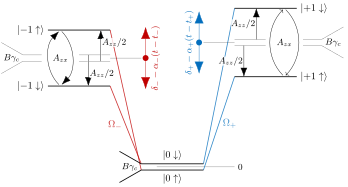
\includegraphics{images/levels.pdf}

}

\caption{\label{fig-levels}Ground state manifold energy levels}

\end{figure}%

The energy levels are depicted in Figure~\ref{fig-levels}, for the
special case of a linear chirp,

\begin{equation}\phantomsection\label{eq-linear-chirp}{
\dot\phi_{\pm}(t) = \alpha_{\pm} (t - t_{\pm})\,,
}\end{equation}

a single carbon atom in the z-x plane (\(A_{zy} = 0\)) and the \(B\)
field aligned to the \(z\) axis (\(\theta = \phi = 0\) in
Equation~\ref{eq-magnetic-field-vector}).

In explicit matrix form, the Hamiltonian for this special case in the
subspace including the electronic spin \(0\) and the \(+1\) subspace is
~{[}\citeproc{ref-AjoySA2018_Hamiltonian.jl}{4}{]}

\begin{equation}\phantomsection\label{eq-hamiltonian-rwa-matrix-plus}{
\hat{H}_{\RWA, +} = \begin{pmatrix}
    \frac{A_{zz}}{2} - \frac{B \gamma_c}{2} - \alpha_{+}(t - t_{+}) + \delta_{+} & \frac{A_{zx}}{2} & \frac{\Omega_{+}(t)}{2} & 0 \\
    \frac{A_{zx}}{2} & -\frac{A_{zz}}{2} + \frac{B \gamma_c}{2} - \alpha_{+} (t - t_{+}) + \delta_{+} & 0 & \frac{\Omega_{+}(t)}{2} \\
    \frac{\Omega_{+}(t)}{2} & 0 & -\frac{B \gamma_c}{2} & 0 \\
    0 & \frac{\Omega_{+}(t)}{2} & 0 & \frac{B \gamma_c}{2}
\end{pmatrix}\,,
}\end{equation}

and, in the subspace with electronic spin \(0\) and \(-1\),

\begin{equation}\phantomsection\label{eq-hamiltonian-rwa-matrix-minus}{
\hat{H}_{\RWA, -} = \begin{pmatrix}
    -\frac{B \gamma_c}{2} & 0 & \frac{\Omega_{-}(t)}{2} & 0\\
    0 & \frac{B \gamma_c}{2} & 0 & \frac{\Omega_{-}(t)}{2} \\
    \frac{\Omega_{-}(t)}{2} & 0 & - \frac{A_{zz}}{2} - \frac{B \gamma_c}{2} - \alpha_{-}(t - t_{-}) + \delta_{-} & \frac{A_{zx}}{2} \\
    0 & \frac{\Omega_{-}(t)}{2} & -\frac{A_{zx}}{2} & \frac{A_{zz}}{2} + \frac{B \gamma_c}{2} - \alpha_{-} (t - t_{-}) + \delta_{-} \\
\end{pmatrix}\,.
}\end{equation}

Note the off-resonant Rabi-cycling in the \(\ket{\pm 1}\) manifolds,
cf.~also Equation~\ref{eq-A-I-matrix}.

\section{Diagonalizing the Hyperfine Interaction}\label{sec-diag}

We can further simplify the Hamiltonian by diagonalizing the projection
of the hyperfine matrix into the nuclear-spin subspace,
Equation~\ref{eq-A-I-matrix}. We note that \(\hat{A}_I^{(n)}\) is
Hermitian, and thus real-valued eigenvalues and a unitary transformation
operator \(\hat{R}^{(n)}\) so that

\begin{equation}\phantomsection\label{eq-eigendecomposition}{
\hat{A}_I^{(n)}
= \hat{R}^{(n)}
    \begin{pmatrix}
    \lambda_{+} & 0 \\ 0 & \lambda_{-}
  \end{pmatrix}
  \hat{R}^{(n)\dagger}
}\end{equation}

This eigendecomposition can be solved analytically
~{[}\citeproc{ref-DiagonalizeHyperfine.jl}{5}{]} with

\begin{equation}\phantomsection\label{eq-analytical-eigenvalues}{
\lambda_{\pm} = \frac{\tr(\hat{A}_I^{(n)})}{2} \pm \sqrt{\frac{\tr^2(\hat{A}_I^{(n)})}{4} - \det(\hat{A}_I^{(n)})}
}\end{equation}

We can see that

\[
\tr(\hat{A}_I^{(n)}) = 0, \qquad
\det(\hat{A}_I^{(n)}) = -\frac{1}{4} {A^{(n)}}^2\,,
\]

with the overall hyperfine magnitude

\begin{equation}\phantomsection\label{eq-A}{
A^{(n)} \equiv \sqrt{{A_{zz}^{(n)}}^2 + {A_{zx}^{(n)}}^2 + {A_{zy}^{(n)}}^2}\,.
}\end{equation}

Thus, we have

\begin{equation}\phantomsection\label{eq-lambda}{
\lambda_{\pm} = \pm A / 2
}\end{equation}

and

\begin{equation}\phantomsection\label{eq-eigendecomposition-A}{
\hat{A}_I^{(n)} = A \, \hat{R}^{(n)} \hat{I}_z^{(n)} \hat{R}^{(n)\dagger}
}\end{equation}

For \(R^{(n)}\), with proper normalization
(\(R^{(n)} {R^{(n)}}^{\dagger} = 𝟙_I^{(n)}\)), we find (temporarily
dropping the superscript \((n)\) on the right-hand-side):

\begin{equation}\phantomsection\label{eq-R}{
\hat{R}^{(n)} = \frac{1}{\sqrt{2}} \begin{pmatrix}
    \frac{A_{zz} + A}{\sqrt{A^2 + A A_{zz}}} & \frac{A_{zz} - A}{\sqrt{A^2 - A A_{zz}}} \\
    \frac{A_{zx} + i A_{zy}}{\sqrt{A^2 + A A_{zz}}} & \frac{A_{zx} + i A_{zy}}{\sqrt{A^2 - A A_{zz}}}
\end{pmatrix}
}\end{equation}

For the total Hamiltonian, we can now define a diagonal frame via the
unitary

\begin{equation}\phantomsection\label{eq-R-total}{
\hat{R} = \hat{R}^{(1)} \otimes \dots \otimes \hat{R}^{(N)}\,.
}\end{equation}

The Hamiltonian in this diagonal frame is

\begin{equation}\phantomsection\label{eq-hamiltonian-diagonal}{
\begin{split}
\hat{H}_{\diag}
& = \hat{R}^\dagger \hat{H}_{\RWA} \hat{R} \\
& = (\hat{\delta} - \hat{\omega}(t)) \otimes 𝟙_I + \sum_{n=1}^{N} \left(A^{(n)} \hat{S}_z \otimes \hat{I}_z^{(n)} - \gamma_c 𝟙_S \otimes \hat{B}_I^{(n)} \right) + \hat{\Omega}(t) \otimes 𝟙_I\,,
\end{split}
}\end{equation}

with \(\hat{B}_I^{(n)}\) defined in Equation~\ref{eq-B-I-matrix}. Any
wave function \(\ket{\tilde{\Psi}(t)}\) in the rotating frame is
transformed into the diagonal frame as
\(\ket{\Psi(t)} = \hat{R}^\dagger \ket{\tilde{\Psi}(t)}\). Note the
dagger, as we have used the common notation for the eigendecomposition
in Equation~\ref{eq-eigendecomposition}, which is the opposite from the
notation used for the rotating frame, cf.
Equation~\ref{eq-H-RWA-general}. The transformation affects the relative
population in the nuclear spins. In the diagonal frame, after
\(\Omega(t)\) has been switched off, the populations remain stable
(since the Hamiltonian is diagonal). In contrast, in the lab/rotating
frame, we would be seeing indefinite off-resonant Rabi-cycling in the
\(\ket{\pm 1}\) manifolds. The transformation \(\hat{R}\) precisely
restores the superposition due to this Rabi cycling.

For the nested-list format in Equation~\ref{eq-nested-list}, this means

\begin{equation}\phantomsection\label{eq-hamiltonian-diagonal-nested-list}{
\hat{H}_{0, \diag} =  \hat{\delta} \otimes 𝟙_I + \sum_{n=1}^{N} \left(A^{(n)} \hat{S}_z \otimes \hat{I}_z^{(n)} - \gamma_c 𝟙_S \otimes \hat{B}_I^{(n)} \right)
}\end{equation}

and \(\hat{H}_{\omega_{-}, \diag}\) \(\hat{H}_{\omega_{+}, \diag}\)
\(\hat{H}_{\Omega_{-}, \diag}\) \(\hat{H}_{\Omega_{+}, \diag}\) as in
Equation~\ref{eq-rwa-hamiltonian-nested-list}; all operators in
\(\HilbertS \otimes \HilbertI\). The only difference between the
rotating frame Hamiltonian in Equation~\ref{eq-rwa-hamiltonian} and the
diagonal frame Hamiltonian is the term
\(\hat{S}_z \otimes \hat{A}_I^{(n)}\) in
Equation~\ref{eq-rwa-hamiltonian} and
Equation~\ref{eq-rwa-hamiltonian-nested-list} being replaced with
\(A^{(n)} \hat{S}_z \otimes \hat{I}_z^{(n)}\) in
Equation~\ref{eq-hamiltonian-diagonal} and
Equation~\ref{eq-hamiltonian-diagonal-nested-list}.

\subsection{Linear Chirp and Single
Carbon}\label{linear-chirp-and-single-carbon-1}

As we did in the rotating frame in
Equation~\ref{eq-hamiltonian-rwa-matrix-plus} and
Equation~\ref{eq-hamiltonian-rwa-matrix-minus}, we can again write out
the Hamiltonian for the \(0/+1\) and \(0/-1\) manifolds under the
assumption of a single nuclear spin and a linear chirp.

\begin{equation}\phantomsection\label{eq-hamiltonian-diag-matrix-plus}{
\hat{H}_{\RWA, +} = \begin{pmatrix}
    \frac{A}{2} - \frac{B \gamma_c}{2} - \alpha_{+}(t - t_{+}) + \delta_{+} &         0        & \frac{\Omega_{+}(t)}{2} & 0 \\
            0        & -\frac{A}{2} + \frac{B \gamma_c}{2} - \alpha_{+} (t - t_{+}) + \delta_{+} & 0 & \frac{\Omega_{+}(t)}{2} \\
    \frac{\Omega_{+}(t)}{2} & 0 & -\frac{B \gamma_c}{2} & 0 \\
    0 & \frac{\Omega_{+}(t)}{2} & 0 & \frac{B \gamma_c}{2}
\end{pmatrix}\,,
}\end{equation}

\begin{equation}\phantomsection\label{eq-hamiltonian-diag-matrix-minus}{
\hat{H}_{\RWA, -} = \begin{pmatrix}
    -\frac{B \gamma_c}{2} & 0 & \frac{\Omega_{-}(t)}{2} & 0\\
    0 & \frac{B \gamma_c}{2} & 0 & \frac{\Omega_{-}(t)}{2} \\
    \frac{\Omega_{-}(t)}{2} & 0 & - \frac{A}{2} - \frac{B \gamma_c}{2} - \alpha_{-}(t - t_{-}) + \delta_{-} &        0         \\
    0 & \frac{\Omega_{-}(t)}{2} &         0         & \frac{A}{2} + \frac{B \gamma_c}{2} - \alpha_{-} (t - t_{-}) + \delta_{-} \\
\end{pmatrix}\,,
}\end{equation}

with the \(A\) given in Equation~\ref{eq-A}.

\section{Mapping between Electronic and Nuclear Spins via Landau-Zener
Crossings}\label{sec-lz}

TODO

After a Landau-Zener transition the probability of population transfer
is ~{[}\citeproc{ref-LandauZener.jl}{6}{]}

\begin{equation}\phantomsection\label{eq-lz-probability}{
P_{LZ} = \exp\left(-2 \pi \frac{\vert\Omega\vert^2}{\vert\alpha\vert^2} \right)
}\end{equation}

\section{Dissipators for the Excited and Metastable
Manifolds}\label{sec-dissipation}

\begin{figure}

\centering{

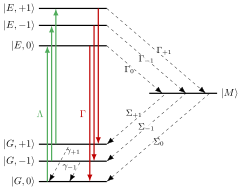
\includegraphics{images/liouville_levels.pdf}

}

\caption{\label{fig-liouville-levels}Level scheme of the combined
optical-electronic subspace}

\end{figure}%

The optical laser field \(\Lambda(t)\) enables incoherent transitions
between the ground state \(\ket{G}\) manifold described above, and the
excited state manifold \(\ket{E}\). We also have a decay channel from
\(\ket{E}\) to \(\ket{G}\) via the metastable state \(\ket{M}\)
(frequently also indicated as \(\ket{S}\) in the literature, but this
might cause confusion), as depicted in
Figure~\ref{fig-liouville-levels}.

The dynamics are described by a master equation in Lindblad form with
the following Lindblad operators:

\begin{itemize}
\tightlist
\item
  \(\hat{A}_{\Lambda} = \sqrt{\Lambda(t)} \ketbra{E}{G} \otimes 𝟙_S \otimes 𝟙_I \,\oplus\, 𝟘_M \otimes 𝟙_I\)
\item
  \(\hat{A}_{\Gamma} = \sqrt{\Gamma}\ketbra{G}{E} \otimes 𝟙_S \otimes 𝟙_I \,\oplus\, 𝟘_M \otimes 𝟙_I\)
\end{itemize}

where \(\ketbra{E}{G}\) and \(\ketbra{G}{E}\) are operators in the
two-dimensional Hilbert space \(\HilbertG \oplus \HilbertE\), cf.~the
second line in Equation~\ref{eq-Hilbert-space-structure}. The first of
the two Lindblad operators above describes the somewhat unusual
\emph{incoherent} excitation of the \(\ket{E}\) manifold. The
time-dependent \(\Lambda(t)\) is not directly supported by the
\texttt{QuantumControl.liouvillian} function. Instead, we construct a
super-operator ~{[}\citeproc{ref-Goerz1312.0111v2}{7}, Appendix B.2{]}

\begin{equation}\phantomsection\label{eq-dissipation-superop}{
L = (\hat{A}^\dagger)^T \otimes \hat{A} - \frac{1}{2} \left(𝟙 \otimes \hat{A}^\dagger \hat{A}\right) - \frac{1}{2} \left((\hat{A}^\dagger \hat{A})^T \otimes 𝟙\right)\,,
}\end{equation}

with \(\hat{A}\) the operator \(\hat{A}_{\Lambda}\) for
\(\sqrt{\Lambda(t)} = 1\) (i.e., without the rate factor). This is done
by calling the \texttt{QuantumControl.liouvillian} function with
\texttt{nothing} as the Hamiltonian and \(\hat{A}\) as the only element
in \texttt{c\_ops}. The resulting \(L\) is then added with a drive
\(\Lambda(t)\) to the Liouvillian super-operator initialized
automatically via the \texttt{QuantumControl.liouvillian} function from
the coherent Hamiltonian previously constructed, the dissipator
\(\hat{A}_{\Gamma}\), and the following further dissipators:

\begin{itemize}
\item
  \(\hat{A}_{\Gamma_{0}} = \sqrt{\Gamma_{0}}\ketbra{M}{E,0} \otimes 𝟙_I\)
\item
  \(\hat{A}_{\Gamma_{-1}} = \sqrt{\Gamma_{-1}}\ketbra{M}{E,-1} \otimes 𝟙_I\)
\item
  \(\hat{A}_{\Gamma_{+1}} = \sqrt{\Gamma_{+1}}\ketbra{M}{E,+1} \otimes 𝟙_I\)
\item
  \(\hat{A}_{\Sigma_{0}} = \sqrt{\Sigma_{0}}\ketbra{G,0}{M} \otimes 𝟙_I\)
\item
  \(\hat{A}_{\Sigma_{-1}} = \sqrt{\Sigma_{-1}}\ketbra{G,-1}{M} \otimes 𝟙_I\)
\item
  \(\hat{A}_{\Sigma_{+1}} = \sqrt{\Sigma_{+1}}\ketbra{G,+1}{M} \otimes 𝟙_I\)
\item
  \(\hat{A}_{\gamma_{+1}} = \sqrt{\gamma_{+1}}\ketbra{G,0}{G,+1} \otimes 𝟙_I\)
\item
  \(\hat{A}_{\gamma_{-1}} = \sqrt{\gamma_{-1}}\ketbra{G,0}{G,-1} \otimes 𝟙_I\)
\end{itemize}

The last two operators are under the assumption that spontaneous decay
of the electronic spin occurs only in the \(\ket{G}\) manifold, as
indicated in Figure~\ref{fig-liouville-levels}; if that decay also
occurred in the \(\ket{E}\) manifold, the corresponding terms
\(\ketbra{E,0}{E,\pm1}\) would have to be added to
\(\hat{A}_{\gamma_{\pm1}}\). All of the above decay operators follow the
structure of the third line in
Equation~\ref{eq-Hilbert-space-structure}.

\section{References}\label{references}

\phantomsection\label{refs}
\begin{CSLReferences}{0}{0}
\bibitem[\citeproctext]{ref-AjoySA2018}
\CSLLeftMargin{{[}1{]} }%
\CSLRightInline{A. Ajoy et al.,
\href{https://doi.org/10.1126/sciadv.aar5492}{Orientation-independent
room temperature optical \(^{13}\){C} hyperpolarization in powdered
diamond}, Sci. Adv. \textbf{4}, (2018).}

\bibitem[\citeproctext]{ref-MultiCarbon.jl}
\CSLLeftMargin{{[}2{]} }%
\CSLRightInline{M. H. Goerz,
\href{https://github.com/ARLQCI/2025-02_C13_Polarization_Hamiltonian}{The
{Hamiltonian} for 1000 carbon atoms surrounding an {NV} center},
\texttt{MultiCarbon.jl} Pluto Notebook in
\texttt{2025-02\_C13\_Polarization\_Hamiltonian} (2025).}

\bibitem[\citeproctext]{ref-RWA_electronic_spin_system.jl}
\CSLLeftMargin{{[}3{]} }%
\CSLRightInline{M. H. Goerz,
\href{https://github.com/ARLQCI/2025-02_C13_Polarization_Hamiltonian}{{Performing
the RWA on the electronic spin system}},
\texttt{RWA\_electronic\_spin\_system.jl} Pluto Notebook in
\texttt{2025-02\_C13\_Polarization\_Hamiltonian} (2025).}

\bibitem[\citeproctext]{ref-AjoySA2018_Hamiltonian.jl}
\CSLLeftMargin{{[}4{]} }%
\CSLRightInline{M. H. Goerz,
\href{https://github.com/ARLQCI/2025-02_C13_Polarization_Hamiltonian}{{The
Hamiltonian of the "¹³C hyperpolarization in diamond" paper}},
\texttt{AjoySA2018\_Hamiltonian.jl} Pluto Notebook in
\texttt{2025-02\_C13\_Polarization\_Hamiltonian} (2025).}

\bibitem[\citeproctext]{ref-DiagonalizeHyperfine.jl}
\CSLLeftMargin{{[}5{]} }%
\CSLRightInline{M. H. Goerz,
\href{https://github.com/ARLQCI/2025-02_C13_Polarization_Hamiltonian}{{Diagonalizing
the Hyperfine Interaction}}, \texttt{DiagonalizeHyperfine.jl} Pluto
Notebook in \texttt{2025-02\_C13\_Polarization\_Hamiltonian} (2025).}

\bibitem[\citeproctext]{ref-LandauZener.jl}
\CSLLeftMargin{{[}6{]} }%
\CSLRightInline{M. H. Goerz,
\href{https://github.com/goerz-research/2025-02-04_Landau_Zener}{Review
of landau zener transitions}, \texttt{LandauZener.jl} Pluto Notebook in
\texttt{2025-02-04\_Landau\_Zener} (2025).}

\bibitem[\citeproctext]{ref-Goerz1312.0111v2}
\CSLLeftMargin{{[}7{]} }%
\CSLRightInline{M. H. Goerz, D. M. Reich, and C. P. Koch,
\href{https://doi.org/10.48550/arXiv.1312.0111v2}{Optimal control theory
for a unitary operation under dissipative evolution}, arXiv:1312.0111v2
(2013).}

\end{CSLReferences}



\end{document}
